\documentclass{beamer}
\usepackage[utf8]{inputenc}
\usepackage{amsmath,amssymb}
\usepackage{graphicx}
\usepackage{epstopdf}
\usepackage[listings,theorems]{tcolorbox}
\usepackage{tikz}
\usepackage{pgf}
\usepackage[customcolors,shade]{hf-tikz}
\setbeamersize{text margin left=5mm,text margin right=5mm} 

\usetikzlibrary{positioning,shapes}
\usetikzlibrary{shapes.geometric,arrows,automata,tikzmark}
\usetikzlibrary{arrows,decorations.pathmorphing}
\tikzstyle{io} = [trapezium, trapezium left angle=70, trapezium right angle=110, minimum width=3cm, minimum height=1cm, text centered, draw=black, fill=blue!30]
\tikzstyle{process} = [rectangle, minimum width=3cm, minimum height=1cm, text centered, draw=black, fill=orange!30]
\tikzstyle{decision} = [diamond, minimum width=3cm, minimum height=1cm, text centered, draw=black, fill=green!30]
\tikzstyle{arrow} = [thick,->,>=stealth]

%Information to be included in the title page:
\title{Optimización de la estructura electrónica del átomo de Be}
\author{A. Mendez}
%\institute{Overleaf}
\date{\today} % It's always today!

\begin{document}
\frame{\titlepage}
%%%%%%%%%%%%%%%%%%%%%%%%%%%%%%%%%%%%%%%%%%%%%%%%%%%%%%%%%%%%%%%%%%%%%%%%
\begin{frame}
\end{frame}
%%%%%%%%%%%%%%%%%%%%%%%%%%%%%%%%%%%%%%%%%%%%%%%%%%%%%%%%%%%%%%%%%%%%%%%%
\begin{frame}
\end{frame}
%%%%%%%%%%%%%%%%%%%%%%%%%%%%%%%%%%%%%%%%%%%%%%%%%%%%%%%%%%%%%%%%%%%%%%%%
\begin{frame}
\frametitle{Variables importantes en la optimización de Be}
\begin{itemize}
\item Configuraciones en CI
\item Tipo de potencial modelo $V_{nl}$ 
      $\rightarrow$ parámetros $\lambda_{nl}$ 
\item Potencial de polarización $V_{\textrm{pol}}(r)$ 
      $\rightarrow$ parámetros $\alpha,r_{\mathrm{cut}}$ 
\end{itemize}
\end{frame}
%%%%%%%%%%%%%%%%%%%%%%%%%%%%%%%%%%%%%%%%%%%%%%%%%%%%%%%%%%%%%%%%%%%%%%%%
\begin{frame}
\frametitle{Optimización del potencial de polarización}

\begin{tikzpicture}[remember picture, overlay]
 \tikzset{shift={(current page.center)},xshift=0cm,yshift=0cm}

 \node<1> (initer) {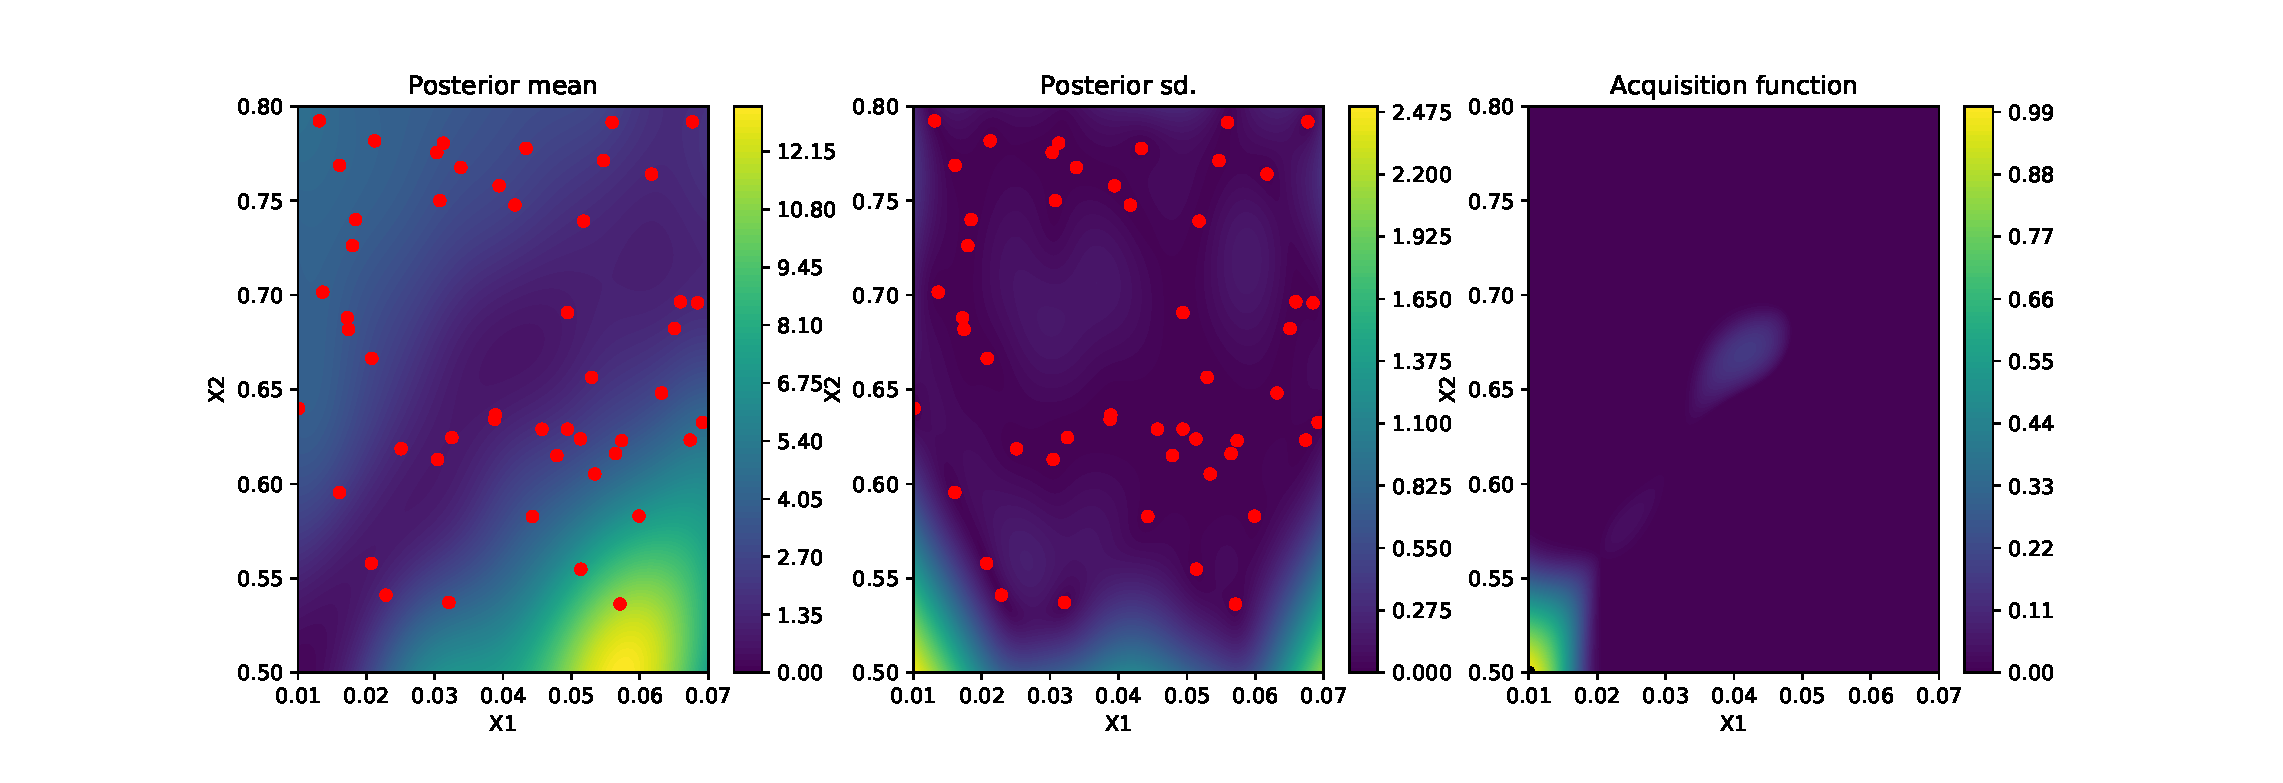
\includegraphics[width=\textwidth]{figures/seed1/space1/polparam_50_0.eps}};
 \node<1> (inipar) at (initer) [xshift=0cm,yshift=2.3cm] {$initer=50\quad\&\quad maxevals=0$};
 \node<1> (inicost) at (initer) [xshift=0cm,yshift=-2.3cm] {$J_{\textrm{min}}=0.8898$ at $\alpha,r_{\textrm{cut}}=[0.0304, 0.6129]$};

 \node<2> (eval10) {\includegraphics[width=\textwidth]{figures/seed1/space1/polparam_50_10.eps}};
 \node<2> (inipar) at (eval10) [xshift=0cm,yshift=2.3cm] {$initer=50\quad\&\quad maxevals=10$};
 \node<2> (inicost) at (eval10) [xshift=0cm,yshift=-2.3cm] {$J_{\textrm{min}}=0.8898$ at $\alpha,r_{\textrm{cut}}=[0.0304, 0.6129]$};

 \node<3> (eval20) {\includegraphics[width=\textwidth]{figures/seed1/space1/polparam_50_20.eps}};
 \node<3> (inipar) at (eval20) [xshift=0cm,yshift=2.3cm] {$initer=50\quad\&\quad maxevals=20$};
 \node<3> (inicost) at (eval20) [xshift=0cm,yshift=-2.3cm] {$J_{\textrm{min}}=0.8898$ at $\alpha,r_{\textrm{cut}}=[0.0304, 0.6129]$};

 \node<4> (eval30) {\includegraphics[width=\textwidth]{figures/seed1/space1/polparam_50_30.eps}};
 \node<4> (inipar) at (eval30) [xshift=0cm,yshift=2.3cm] {$initer=50\quad\&\quad maxevals=30$};
 \node<4> (inicost) at (eval30) [xshift=0cm,yshift=-2.3cm] {$J_{\textrm{min}}=0.8898$ at $\alpha,r_{\textrm{cut}}=[0.0304, 0.6129]$};

 \draw<1-4>[yellow,line width=0.5mm] (-3.7,-0.36) circle (0.1cm);

 \node<5> (eval40) {\includegraphics[width=\textwidth]{figures/seed1/space1/polparam_50_40.eps}};
 \node<5> (inipar) at (eval40) [xshift=0cm,yshift=2.3cm] {$initer=50\quad\&\quad maxevals=40$};
 \node<5> (inicost) at (eval40) [xshift=0cm,yshift=-2.3cm] {$J_{\textrm{min}}=0.8878$ at $\alpha,r_{\textrm{cut}}=[0.0265, 0.5975]$};

 \draw<5>[yellow,line width=0.5mm] (-3.83,-0.51) circle (0.1cm);

 \node<6> (eval50) {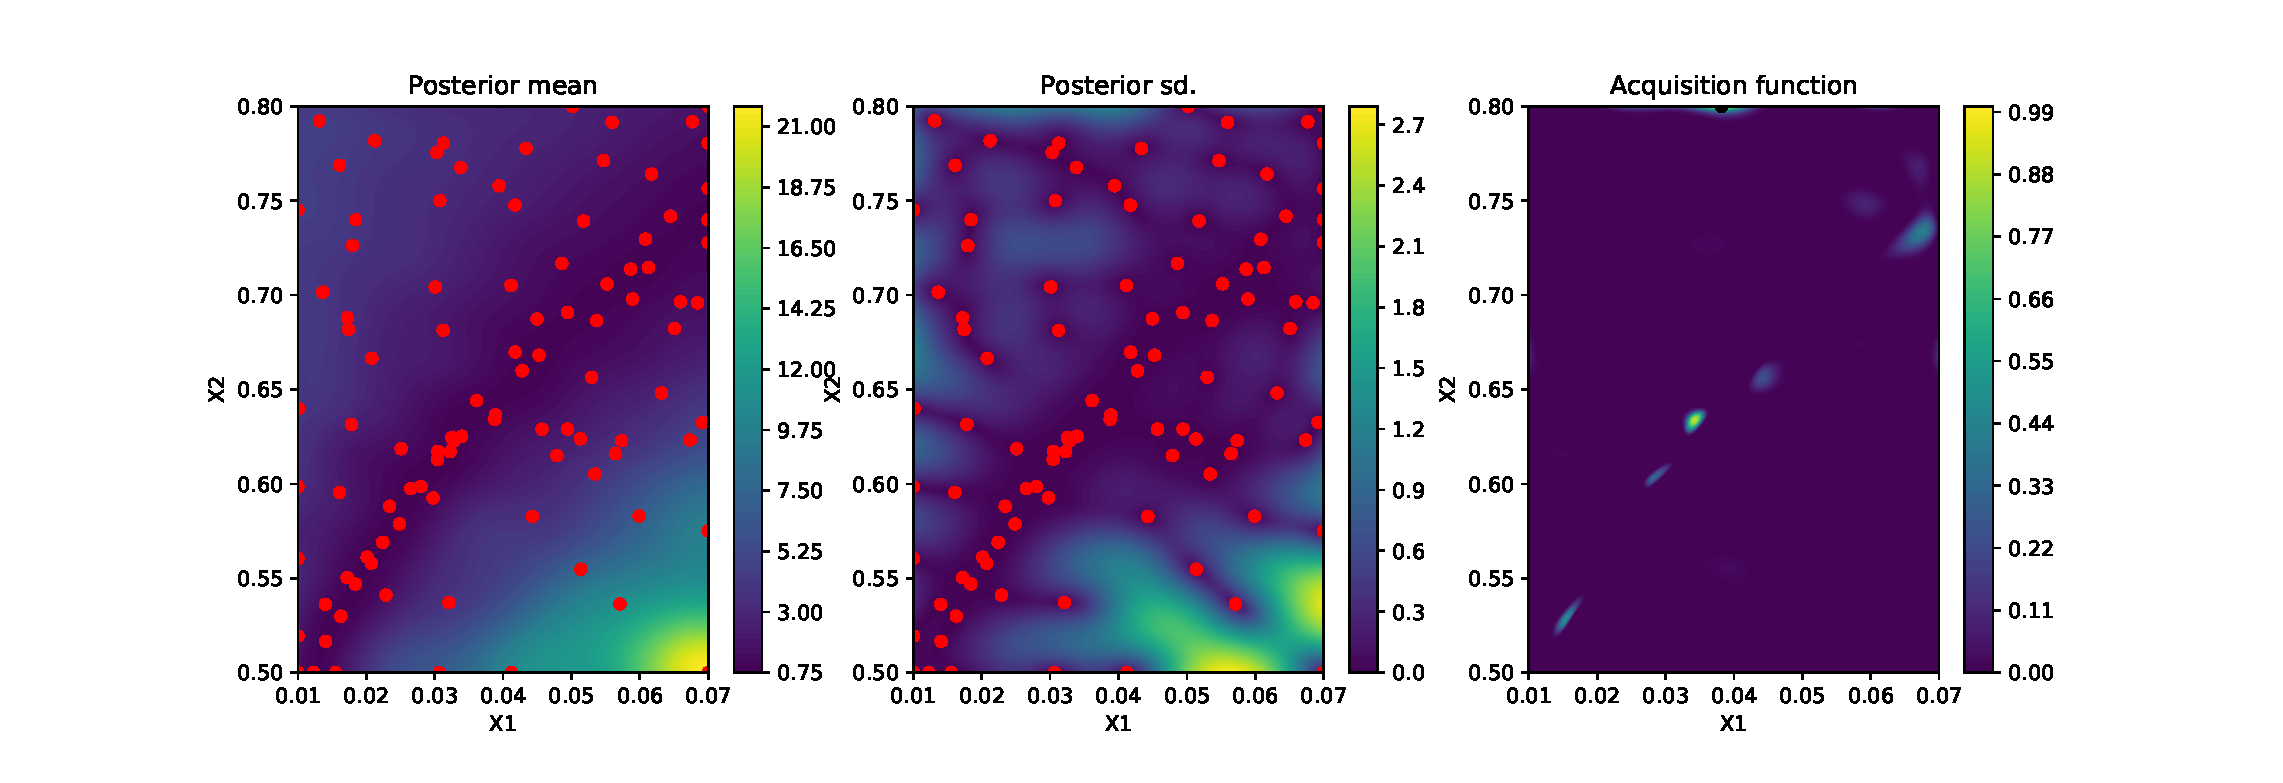
\includegraphics[width=\textwidth]{figures/seed1/space1/polparam_50_50.eps}};
 \node<6> (inipar) at (eval50) [xshift=0cm,yshift=2.3cm] {$initer=50\quad\&\quad maxevals=50$};
 \node<6> (inicost) at (eval50) [xshift=0cm,yshift=-2.3cm] {$J_{\textrm{min}}=0.8804$ at $\alpha,r_{\textrm{cut}}=[0.0163, 0.5299]$};

 \node<7> (eval60) {\includegraphics[width=\textwidth]{figures/seed1/space1/polparam_50_60.eps}};
 \node<7> (inipar) at (eval60) [xshift=0cm,yshift=2.3cm] {$initer=50\quad\&\quad maxevals=60$};
 \node<7> (inicost) at (eval60) [xshift=0cm,yshift=-2.3cm] {$J_{\textrm{min}}=0.8804$ at $\alpha,r_{\textrm{cut}}=[0.0163, 0.5299]$};

 \node<8> (eval130) {\includegraphics[width=\textwidth]{figures/seed1/space1/polparam_50_130.eps}};
 \node<8> (inipar) at (eval130) [xshift=0cm,yshift=2.3cm] {$initer=50\quad\&\quad maxevals=130$};
 \node<8> (inicost) at (eval130) [xshift=0cm,yshift=-2.3cm] {$J_{\textrm{min}}=0.8804$ at $\alpha,r_{\textrm{cut}}=[0.0163, 0.5299]$};

 \draw<6-8>[yellow,line width=0.5mm] (-4.19,-1.19) circle (0.1cm);

\end{tikzpicture}

\end{frame}
%%%%%%%%%%%%%%%%%%%%%%%%%%%%%%%%%%%%%%%%%%%%%%%%%%%%%%%%%%%%%%%%%%%%%%%%
\begin{frame}
\frametitle{Optimización del potencial de polarización - parte 2}

\begin{tikzpicture}[remember picture, overlay]
 \tikzset{shift={(current page.center)},xshift=0cm,yshift=0cm}

 \node<1> (initer) {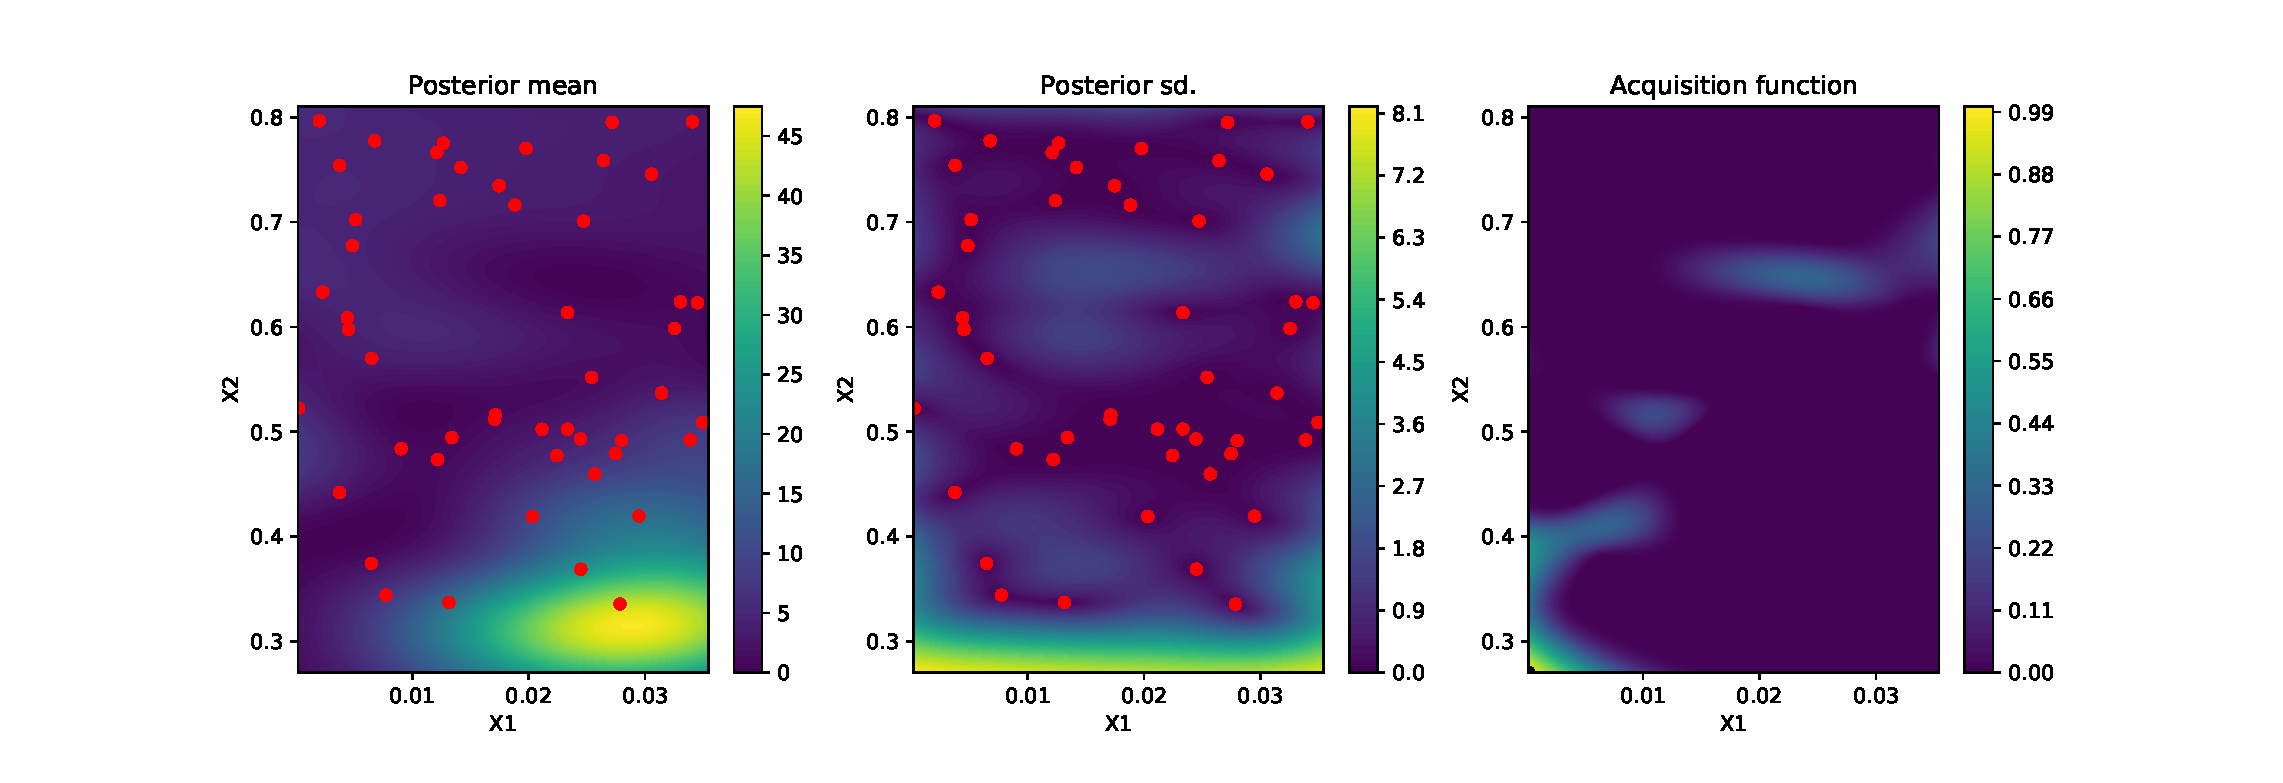
\includegraphics[width=\textwidth]{figures/seed1/space2/polparam_50_0.eps}};
 \node<1> (inipar) at (initer) [xshift=0cm,yshift=2.3cm] {$initer=50\quad\&\quad maxevals=0$};
 \node<1> (inicost) at (initer) [xshift=0cm,yshift=-2.3cm] {$J_{\textrm{min}}=0.8785$ at $\alpha,r_{\textrm{cut}}=[0.0140,0.5079]$};

 \draw<1>[yellow,line width=0.5mm] (-3.62,-0.24) circle (0.1cm);

 \node<2> (eval10) {\includegraphics[width=\textwidth]{figures/seed1/space2/polparam_50_10.eps}};
 \node<2> (inipar) at (eval10) [xshift=0cm,yshift=2.3cm] {$initer=50\quad\&\quad maxevals=10$};
 \node<2> (inicost) at (eval10) [xshift=0cm,yshift=-2.3cm] {$J_{\textrm{min}}=0.8737$ at $\alpha,r_{\textrm{cut}}=[0.0080,0.4446]$};

 \node<3> (eval20) {\includegraphics[width=\textwidth]{figures/seed1/space2/polparam_50_20.eps}};
 \node<3> (inipar) at (eval20) [xshift=0cm,yshift=2.3cm] {$initer=50\quad\&\quad maxevals=20$};
 \node<3> (inicost) at (eval20) [xshift=0cm,yshift=-2.3cm] {$J_{\textrm{min}}=0.8737$ at $\alpha,r_{\textrm{cut}}=[0.0080,0.4446]$};

 \node<4> (eval30) {\includegraphics[width=\textwidth]{figures/seed1/space2/polparam_50_30.eps}};
 \node<4> (inipar) at (eval30) [xshift=0cm,yshift=2.3cm] {$initer=50\quad\&\quad maxevals=30$};
 \node<4> (inicost) at (eval30) [xshift=0cm,yshift=-2.3cm] {$J_{\textrm{min}}=0.8737$ at $\alpha,r_{\textrm{cut}}=[0.0080,0.4446]$};

 \node<5> (eval40) {\includegraphics[width=\textwidth]{figures/seed1/space2/polparam_50_40.eps}};
 \node<5> (inipar) at (eval40) [xshift=0cm,yshift=2.3cm] {$initer=50\quad\&\quad maxevals=40$};
 \node<5> (inicost) at (eval40) [xshift=0cm,yshift=-2.3cm] {$J_{\textrm{min}}=0.8737$ at $\alpha,r_{\textrm{cut}}=[0.0080,0.4446]$};

% \node<6> (eval50) {\includegraphics[width=\textwidth]{figures/seed1/space2/polparam_50_100.eps}};
% \node<6> (inipar) at (eval50) [xshift=0cm,yshift=2.3cm] {$initer=50\quad\&\quad maxevals=100$};
% \node<6> (inicost) at (eval50) [xshift=0cm,yshift=-2.3cm] {$J_{\textrm{min}}=0.8737$ at $\alpha,r_{\textrm{cut}}=[0.0080,0.4446]$};

 \draw<2-5>[yellow,line width=0.5mm] (-3.62,-0.24) circle (0.1cm);

\end{tikzpicture}


\end{frame}
%%%%%%%%%%%%%%%%%%%%%%%%%%%%%%%%%%%%%%%%%%%%%%%%%%%%%%%%%%%%%%%%%%%%%%%%
\begin{frame}
\end{frame}
%%%%%%%%%%%%%%%%%%%%%%%%%%%%%%%%%%%%%%%%%%%%%%%%%%%%%%%%%%%%%%%%%%%%%%%%
\begin{frame}
\end{frame}
%%%%%%%%%%%%%%%%%%%%%%%%%%%%%%%%%%%%%%%%%%%%%%%%%%%%%%%%%%%%%%%%%%%%%%%%
\end{document}
